\documentclass[a4paper, 12pt]{article}
\usepackage[utf8]{inputenc}
\usepackage[french]{babel}
\usepackage[T1]{fontenc}
\usepackage[top=2cm,bottom=2cm,left=2cm,right=2cm]{geometry}
\usepackage{hyperref}
\usepackage{graphicx}
\usepackage{caption}
\usepackage{sectsty}
\usepackage{xcolor}
\usepackage{tabularx}
\usepackage{colortbl}
\usepackage{tkz-graph}
\usepackage{listings}
\usepackage[linesnumbered,ruled,french,onelanguage]{algorithm2e}
\usepackage{tikz}
\usepackage{fancyhdr}
\usepackage{float}

% Pour algorithm2me---------------------------------------------
\SetKwRepeat{Do}{do}{while}%
\makeatletter 
\g@addto@macro{\@algocf@init}{\SetKwInput{KwOut}{Sortie}}
\makeatother
%---------------------------------------------
\captionsetup{position=below}
\hypersetup{pdfborder = 0 0 0}
%---------------------------------------------
% définition des couleurs
\definecolor{color_section}{RGB}{87,68,95}
\definecolor{color_subsection}{RGB}{46,81,159}
\definecolor{color_sub-subsection}{RGB}{121,142,200}
\definecolor{ashgrey}{RGB}{145,120,155}
%---------------------------------------------
% associer les couleurs aux titres de section
\sectionfont{\color{color_section}\underline}
\subsectionfont{\color{color_subsection}\underline}
\subsubsectionfont{\color{color_sub-subsection}\underline}
%---------------------------------------------
% entête
\title{- Rapport de projet - \\ Conception d'un solveur de ricochet robots}
\author{
    \textsc{André} Lorada \\ 
    \textsc{Auvray} Théo \\ 
    Licence 2 informatique - Groupe 1A
}
\date \today
%---------------------------------------------
%entête
\pagestyle{fancy}%
\fancyhf{}%
\fancyfoot[L] {%
	\thepage{} {\raisebox{-0.6ex}{\color{color_section}\fontsize{18}{20}\selectfont\bfseries|}} Rapport de projet -  Conception d'un solveur de ricochet robots%
}%
\fancyhead[L] {\textbf{\nouppercase\leftmark}}%
\setlength{\headheight}{16pt}
\fancyhead[R] {\nouppercase\rightmark}%
%---------------------------------------------
\begin{document}
%%%%%%%%%%%%%%%%%%%%%%%%%%%%%%%%%%%%%%%%%%%%%%%%%%%%%%%%%%%%%%%%%%%%%%%%%%%%%%%%%%%%%%%%%%%%%%%%%%%%%%%%%%%%%%%%%%%%%%%%
% PAGE D'ACCUEIL
\begin{figure}[t]
    
\includegraphics[scale=1]{images/logo.png}
\end{figure}

\maketitle

\begin{figure}[H]
    \centering
    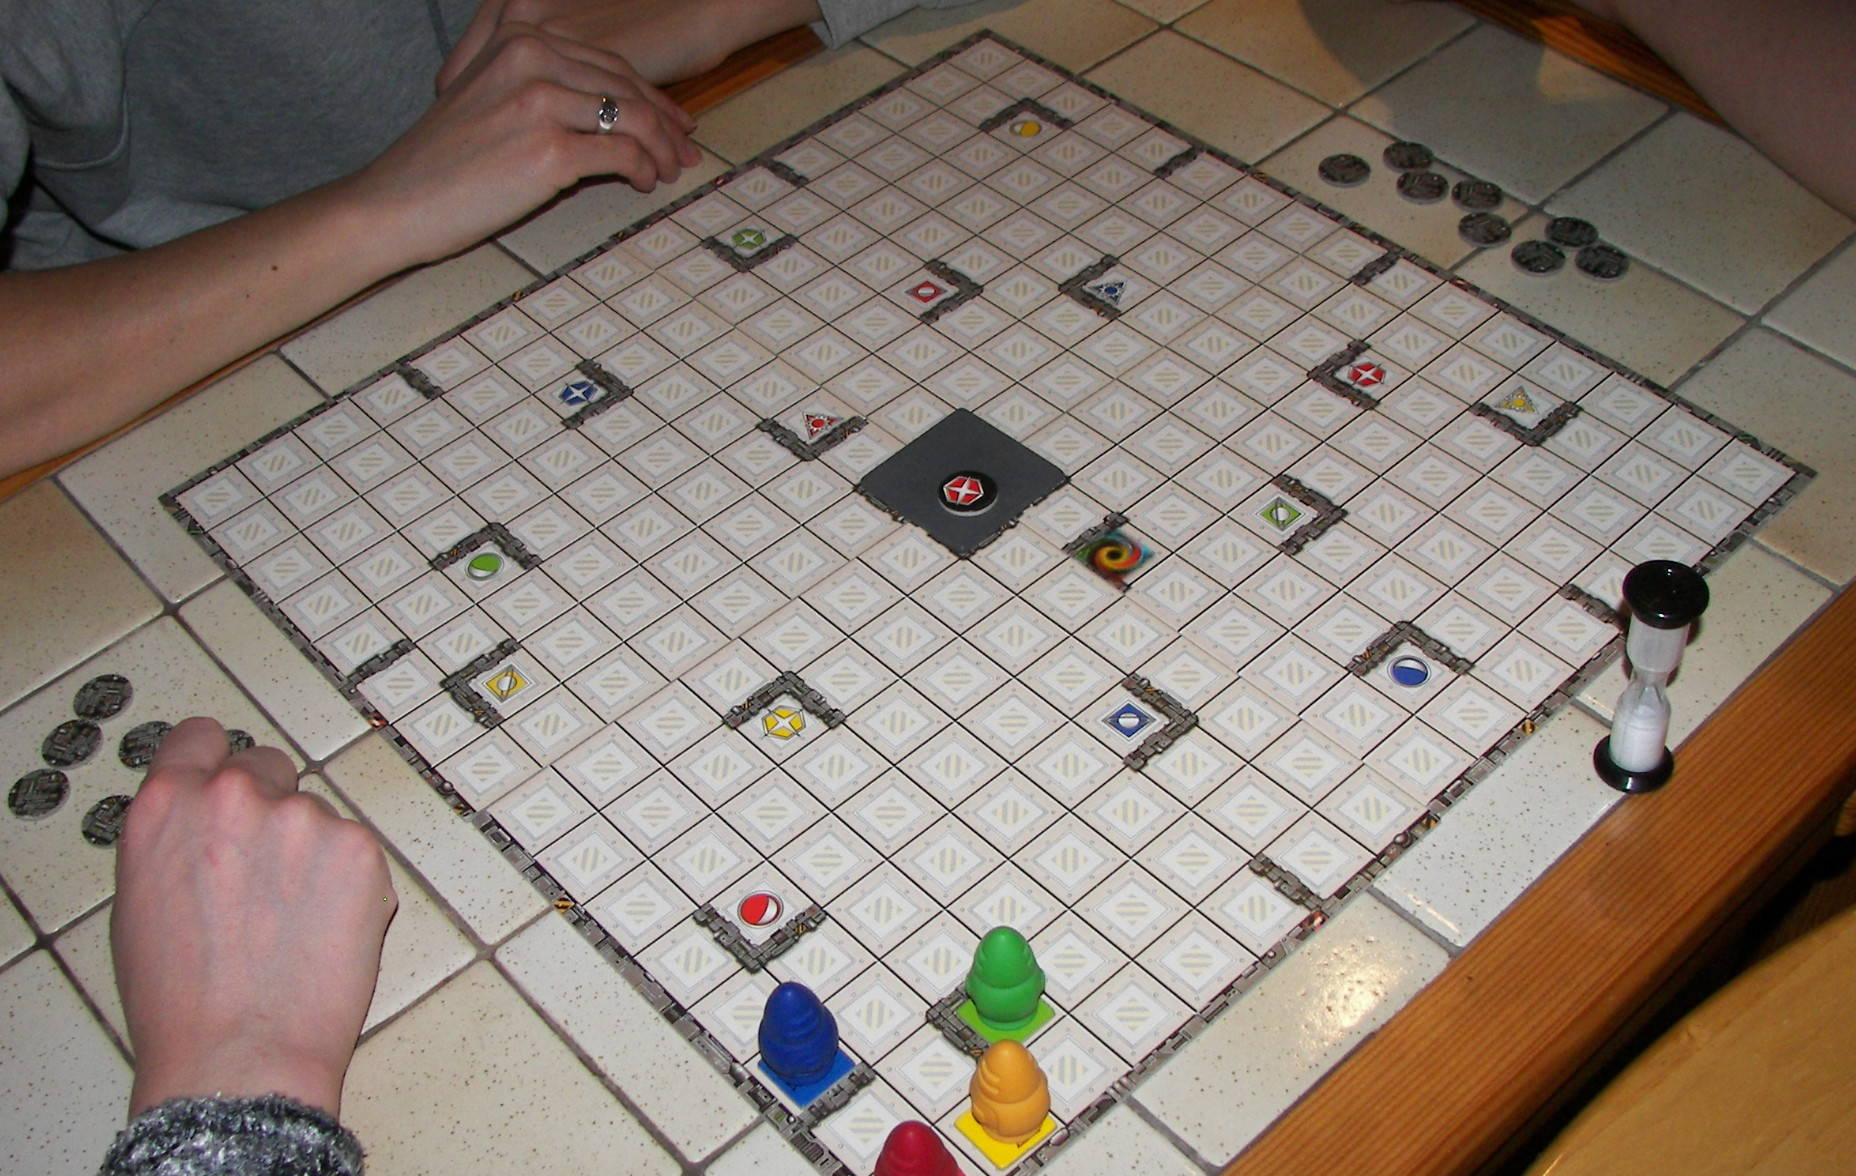
\includegraphics[scale=0.5]{images/ricochetrobot.jpg}
\end{figure}

\newpage %%%%%%%%%%%%%%%%%%%%%%%%%%%%%%%%%%%%%%%%%%%%%%%%%%%%%%%%%%%%%%%%%%%%%%%%%%%%%%%%%%%%%%%%%%%%%%%%%%%%%%%%%%%%%%%%%%%%%%%%
%table des matières

\tableofcontents

\newpage %%%%%%%%%%%%%%%%%%%%%%%%%%%%%%%%%%%%%%%%%%%%%%%%%%%%%%%%%%%%%%%%%%%%%%%%%%%%%%%%%%%%%%%%%%%%%%%%%%%%%%%%%%%%%%%%%%%%%%%%
\section{Introduction}
Le Ricochet Robots est à l'origine un jeu de plateau. D'après Wikipédia\cite{Wikipedia}, ce jeu de société est composé d'un plateau, de tuiles représentant chacune des cases du plateau, et de pions appelés "robots" et "jetons". Différents jetons sont imprimés dans certaines des cases (au nombre de 17). Le jeu commence en piochant un pion "jeton" parmi les 17. La case à aller correspond au symbole du jeton qui a été tiré aléatoirement. La partie est décomposée en tours de jeu, un tour consistant à déplacer les robots sur le plateau afin d'emmener le robot de la même couleur du jeton tiré sur la case correspondante. Les robots ne peuvent que se déplacer qu'en ligne droite jusqu'à rencontrer un obstacle (un robot ou un mur).

    \paragraph{}
    Le Ricochet Robot peut aussi bien être joué seul qu'avec un grand nombre de participants. Le jeton revient à la personne qui aura trouvé la séquence de mouvement qui permettra à un robot donné (parmi quatre), d'atteindre la case, en moins de coups possible dans un délai de temps imparti. La partie se termine lorsque tout les jetons auront été tirés. Le gagnant est la personne qui aura récolté le plus de jetons.
    
    \paragraph{}
    Le but de ce projet à été de développer un programme permettant de trouver une solution optimale pour toute situation du jeu. La conception de ce projet à été réalisée en plusieurs temps:
        \begin{itemize}
            \item Le développement du moteur du jeu suivant les règles du Ricochet Robots
            \item Réalisation d'une interface graphique.
            \item Implantation d'un algorithme de résolution naïf, appelé A*.
            \item Proposer des méthodes d'optimisation de l'algorithme, par soucis de complexité pour être résolu dans de bonnes conditions.
        \end{itemize}

\newpage %%%%%%%%%%%%%%%%%%%%%%%%%%%%%%%%%%%%%%%%%%%%%%%%%%%%%%%%%%%%%%%%%%%%%%%%%%%%%%%%%%%%%%%%%%%%%%%%%%%%%%%%%%%%%%%%%%%%%%%%

\section{Organisation du projet}

    \subsection{Gestion du projet}

		Afin de faciliter la communication et le bon déroulement de la conception de notre jeu, divers moyens ont été mis en oeuvre.

        \subsubsection{Hébergement du code}
        
            Afin de faciliter la gestion du projet, nous avons utilisé à la fois \href{https://forge.info.unicaen.fr/}{la Forge} d’Unicaen et \href{https://github.com/}{Github} qui permettent de créer et d’administrer des dépôts sous Git très facilement par l’intermédiaire d’une interface web. D’autres fonctionnalités sont disponibles  sur ces plate-formes comme une gestion des permissions, une visualisation des différents commits, la visualisation de l’activité du projet, etc. L'utilisation supplémentaire de \href{https://github.com/}{Github} permettait de centraliser les projets de la licence sur une seule plate-forme ainsi que l'utilisation de "Webhooks" (envoi de notifications sur \href{https://discordapp.com/}{Discord} lors de la mise en ligne d'une fonctionnalité).
            
		\subsubsection{Gestionnaire de version}

			Nous avons utilisé un gestionnaire de version afin de permettre la centralisation du code et rendre le travail en équipe bien plus efficace. Nous avons opté pour Git, qui est un gestionnaire de version que nous avons utilisé dans un précédent projet. L'utilisation de Git rend l'utilisation des branches plus facile, permet de faire des commits sans pour autant être connecté sur le serveur. Cela permet de faire plus de commits, qui sont enregistrés localement et de les envoyer sur le serveur en une seule fois, au moment où nous sommes sûrs que la fonctionnalité ajoutée fonctionne. Git permet également de transférer facilement son code vers un autre hébergeur en ajoutant simplement une "route" (remote), tout en conservant la totalité des commits réalisés.

		\subsubsection{Trello}

			Concernant la répartition et le listage du travail à effectuer, nous avons fait le choix d'utiliser \href{https://trello.com/}{Trello}, une plate-forme qui nous permet l'utilisation de tableaux afin de planifier le projet.

			\begin{figure}[H]
				\centering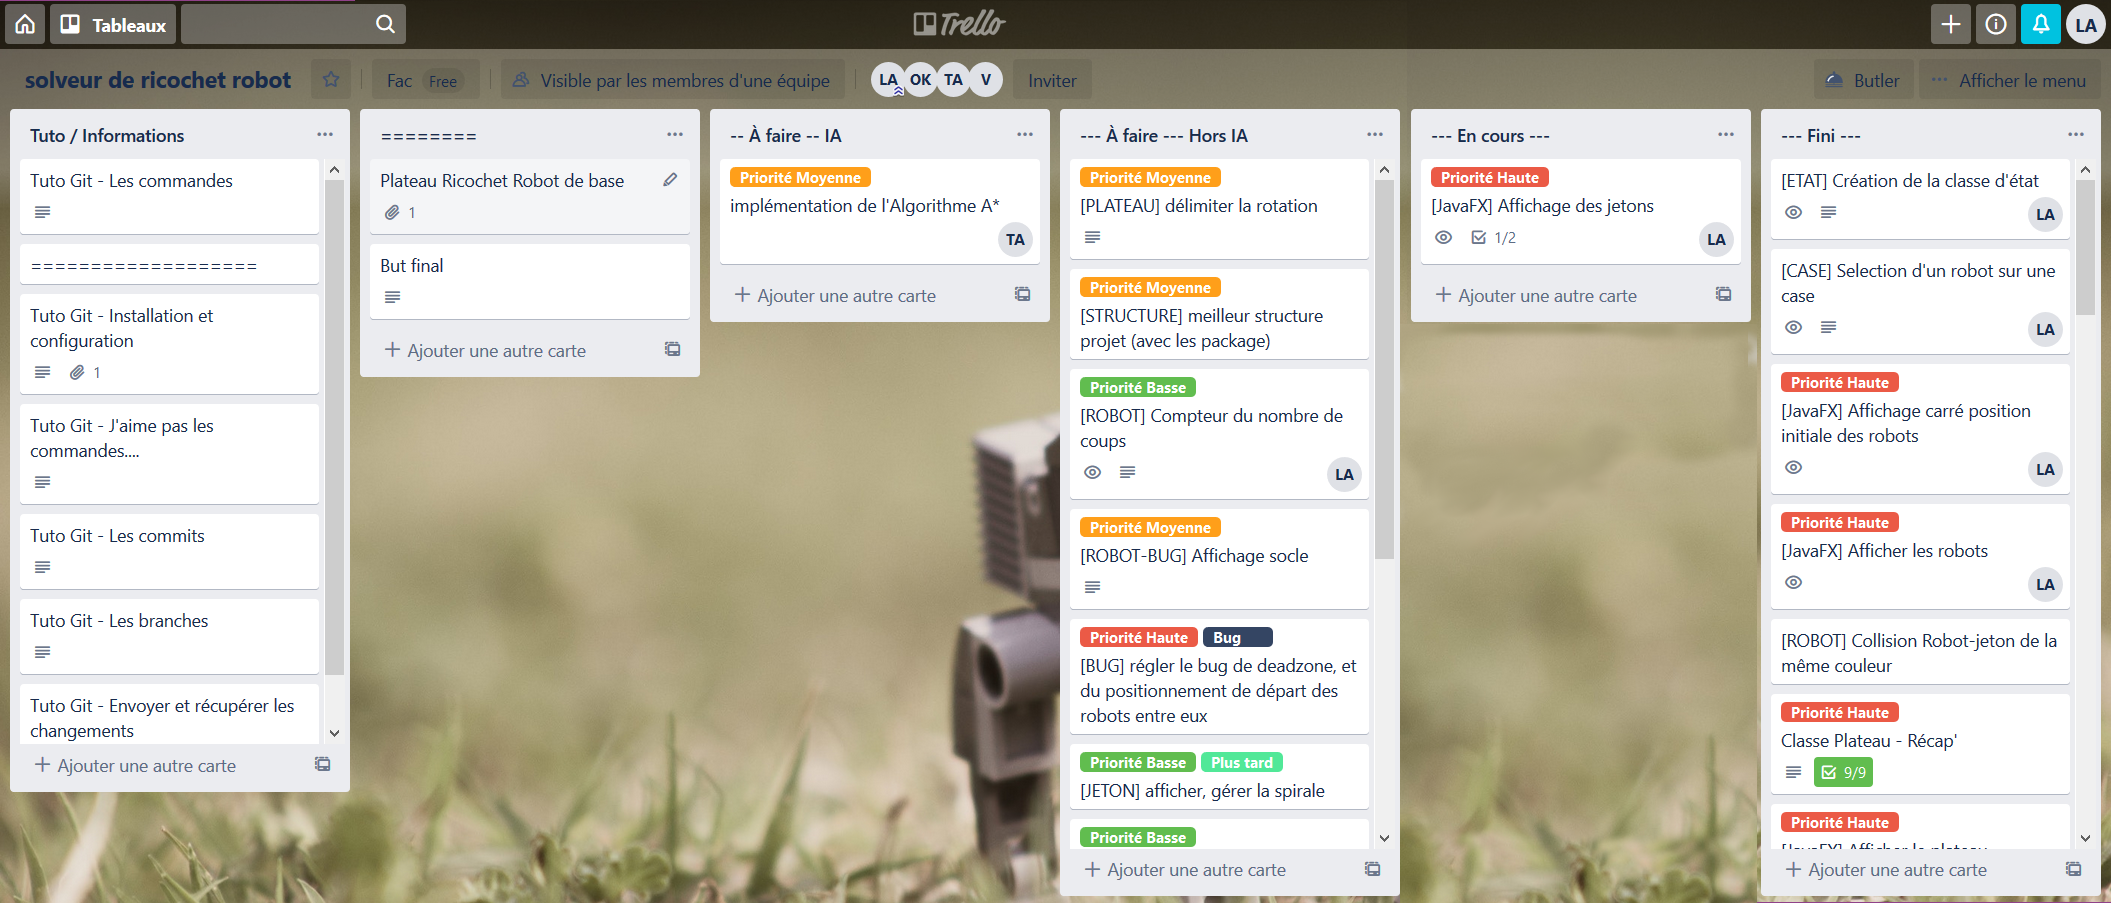
\includegraphics[width=0.95\textwidth]{images/trello.png}
				\caption{Notre tableau Trello}
			\end{figure}

			Ainsi, comme nous pouvons le constater sur l'image ci-dessus, les différentes tâches passent par différents états appelés "\textit{À faire}", "\textit{En cours}", "\textit{À modifier et à vérifier}", et "\textit{Fini}".

			La colonne "\textit{À modifier et à vérifier}" est utilisée lorsqu'une tâche est réalisée, mais doit être modifiée (car elle n'est pas optimale) ou doit être soumise à évaluation et/ou relecture. Cela permet d'éviter d'éventuels bugs par la suite mais aussi de garder une cohérence au travers du code. Lorsque cette tâche est modifiée et/ou vérifiée, elle est déplacée dans la colonne "\textit{Fini}".

		\subsubsection{Discord}

			Afin de faciliter la communication au sein du groupe, nous avons utilisé le service de messagerie \href{https://discordapp.com/}{Discord}  car tous les membres du groupe l'utilisaient déjà de manière personnelle. Ce service permet de parler par le biais de "serveurs" gratuits dans lesquels nous pouvons ajouter des salons textuels ou des salons vocaux à volonté.

			\begin{figure}[H]
				\centering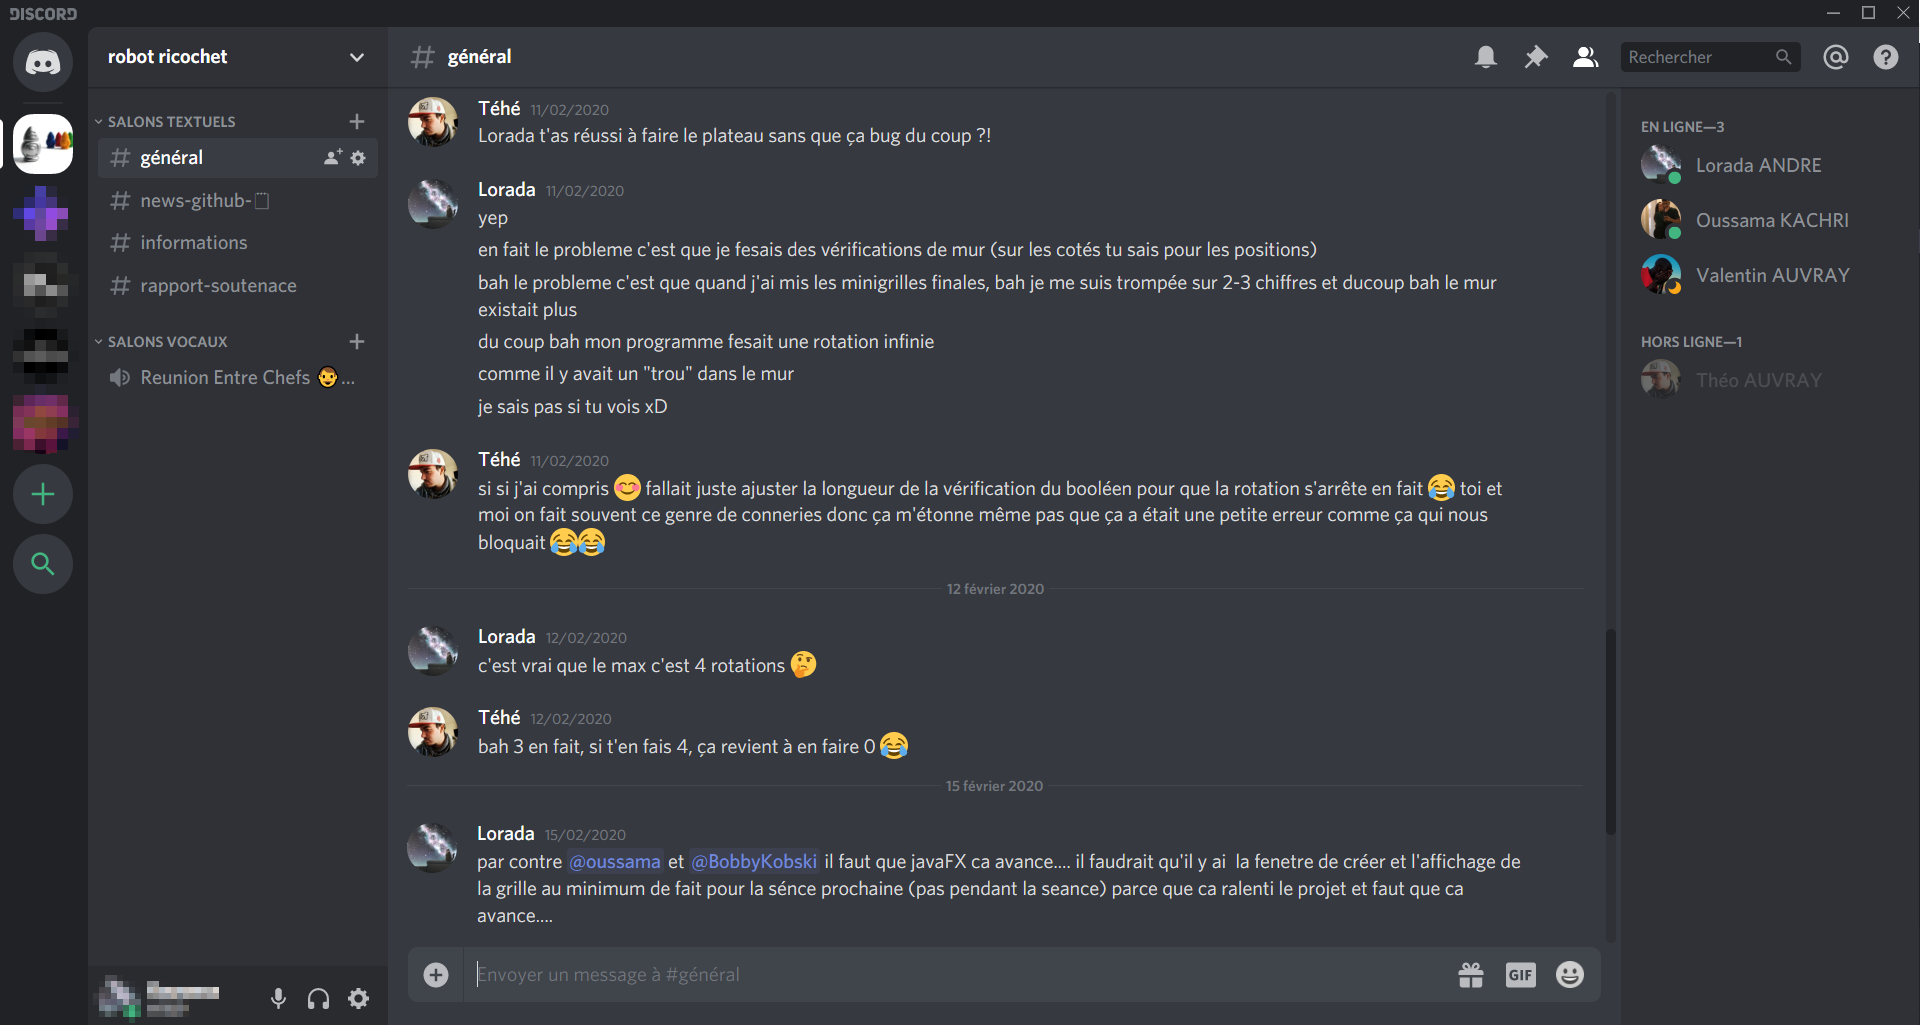
\includegraphics[scale=1]{images/discord.png}
				\caption{Notre serveur Discord}
			\end{figure}
			
			 Ainsi, nous avions un salon de discussion, nommé "\textit{informations}". Comme son nom l'indique, il permet de transmettre des messages importants sur ce qui a été fait, sur des changements importants concernant le projet, etc. un deuxième se nommant "\textit{news-Github}" servait à recevoir une notification dès qu'une personne ajoutait du code sur \href{https://github.com/}{Github}, afin de connaître l'avancement de chaque personne sans pour autant devoir aller sur les hébergeurs, ou bien pour qu'une personne sache à quel moment elle devait reprendre le relais sur une fonctionnalité. Le troisième salon se nommant"\textit{général}" était utilisé pour les discutions beaucoup plus générales. Sur ce salon, nous pouvions discuter du projet, de certains choix à faire, ou bien demander de l'aide ou aider des membres en difficulté.
			
			
    \subsection{Répartition des tâches}
    
    \begin{center}
        \begin{tabular}{|p{7cm}|>{\centering\arraybackslash}p{4cm}|>{\centering\arraybackslash}p{4cm}|}
            \hline
                Tâches & Lorada & Théo \\
            \hline %................
                \rowcolor{ashgrey} Plateau  & &\\
                 Création de la classe Plateau & X & \\
                 \hline
                 Création des quarts de plateau & X & \\
                 \hline
                 Assemblage des quarts de plateau &  & X \\
                 \hline
                 Génération aléatoire du plateau & X & \\
                 \hline
                 Rotation des quarts de plateau & X & \\
                 \hline
                 Affichage graphique du plateau & X & \\
            \hline %................
                \rowcolor{ashgrey} Robot  & &\\
                 Création de la classe &  & X \\
                 \hline
                 Positionnement aléatoire des robots & X &\\
                 \hline
                 Collisions des robots avec les éléments & X &\\
                 \hline 
                 Déplacement des robots & X &\\
                 \hline 
                 Sélection d'un robot & X &\\
                 \hline
                 Affichage des robots et des socles & X & \\
            \hline %................
                \rowcolor{ashgrey} Jeton  & &\\
                 Création de la classe Jeton & X & \\
                \hline
                Génération aléatoire du jeton tiré & & X\\
                \hline
                Affichage graphique du jeton tiré & X & \\
             \hline %................
                \rowcolor{ashgrey} Case  & &\\
                 Création de la classe Case & X & \\
                 \hline
                 Positionnement des cases & X & \\
                  \hline
                Rotation des cases & X & \\
                \hline
                 Affichage graphique des cases & X & \\
            \hline %................
                \rowcolor{ashgrey} Case Jeton   & &\\
                Création de la classe Case Jeton & X & \\
                \hline
                Positionnement des jetons & & X\\
                \hline
                Rotation des cases jeton & X & \\
                 \hline
                Affichage graphique des cases jetons & X & \\
            \hline %................
                \rowcolor{ashgrey} Pattern Observer  & &\\
                Implémentation du pattern observer & X & \\   
             \hline %................
                \rowcolor{ashgrey} Score  & &\\
                 Création de la classe Score & X & \\
                 \hline
                Création du système de score & X & \\   
            \hline %................
                \rowcolor{ashgrey} State & &\\
                 Création de la classe State & X & \\
                 \hline
                Création de l'état initial du jeu & X & \\   
                \hline
                Déplacement du robot avec le clavier & X &\\
                \hline
                Séléction du robot qui doit jouer & X &\\
                \hline
                Définition de l'état gagnant & X &\\
            \hline %................
             \rowcolor{ashgrey} Algorithme A* & &\\
                Algorithme BFS & X , partiellement fontionnel & \\   
                \hline
                 Sortie Anticipée & X &\\  
                \hline
                 Mise en place de l'heuristique & manque de temps &\\  
                \hline
             \hline %................
             \rowcolor{ashgrey} Rapport & &\\
             Rédaction du rapport & X & \\
            \hline %................
        \end{tabular}
    \end{center}
    
\newpage %%%%%%%%%%%%%%%%%%%%%%%%%%%%%%%%%%%%%%%%%%%%%%%%%%%%%%%%%%%%%%%%%%%%%%%%%%%%%%%%%%%%%%%%%%%%%%%%%%%%%%%%%%%%%%%%%%%%%%%%

\section{Architecture du projet}
    \subsection{Arborescence du projet}
    
        Le projet est structuré de la manière suivante:
        
        \begin{figure}[H]
    		\centering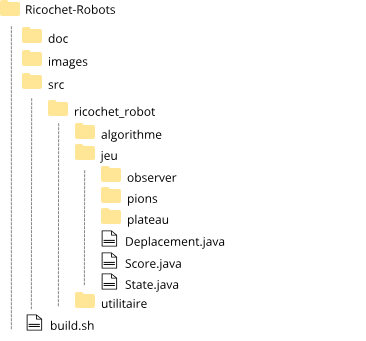
\includegraphics[width=0.5\textwidth]{images/structureprojet.png}
    		\caption{Arborescence du projet}
    	\end{figure}
    	
    	\paragraph{}
    	Á la racine de ce projet, nous y retrouvons:
    	
    	\begin{description}
    	    \item [doc:] contient ce rapport et prochainement le diaporama pour la soutenance.
    	    \item [images:] contient l'ensemble des images utilisées pour la partie interface graphique du jeu.
    	    \item [src:] contient le code source du projet.
    	    \item [build.sh:] le script de compilation du projet.
    	\end{description}
    	
    \subsection{Architecture du programme}
    
        \subsubsection{Diagramme des packages}
            
            \paragraph{}
             Le code source est organisé dans différents packages:
             
            \begin{description}
            \item[algorithme:] contient les classes relatives à l'implémentation de l'algorithme A*.
                 \item[jeu:] contient tout les éléments relatifs au jeu.
                 \begin{description}
            	    \item[observer:] regroupe les différentes classes utilisées pour l'implémentation du pattern observer.
            	    \item[pions:] contient les classes représentants les éléments mobiles du Ricochet Robots, correspondant au robot et au jeton  
            	    \item[plateau:] contient les classes relatives à la création du plateau
        	    \end{description}
                 \item[utilitaire:] contient une classe utilitaire.
             \end{description}
             
            \begin{figure}[H]
                \centering
                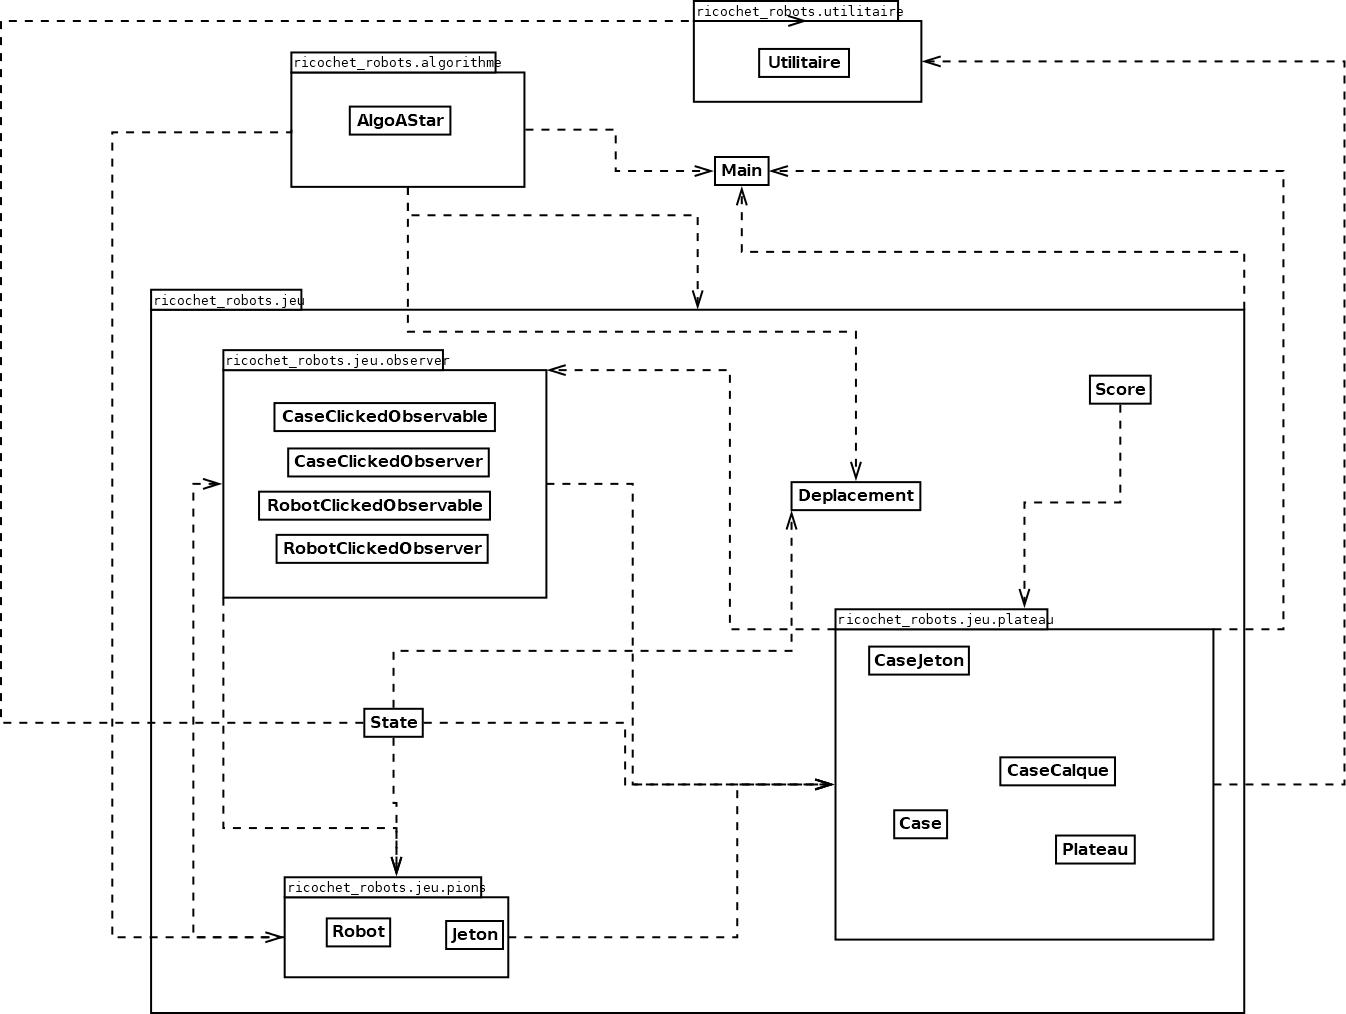
\includegraphics[scale=0.3]{images/diagrammePackage.png}
                 \caption{Diagramme des packages}
            \end{figure}

            \newpage
            
        \subsubsection{Diagramme des classes}
        
            \begin{figure}[H]
                \centering
                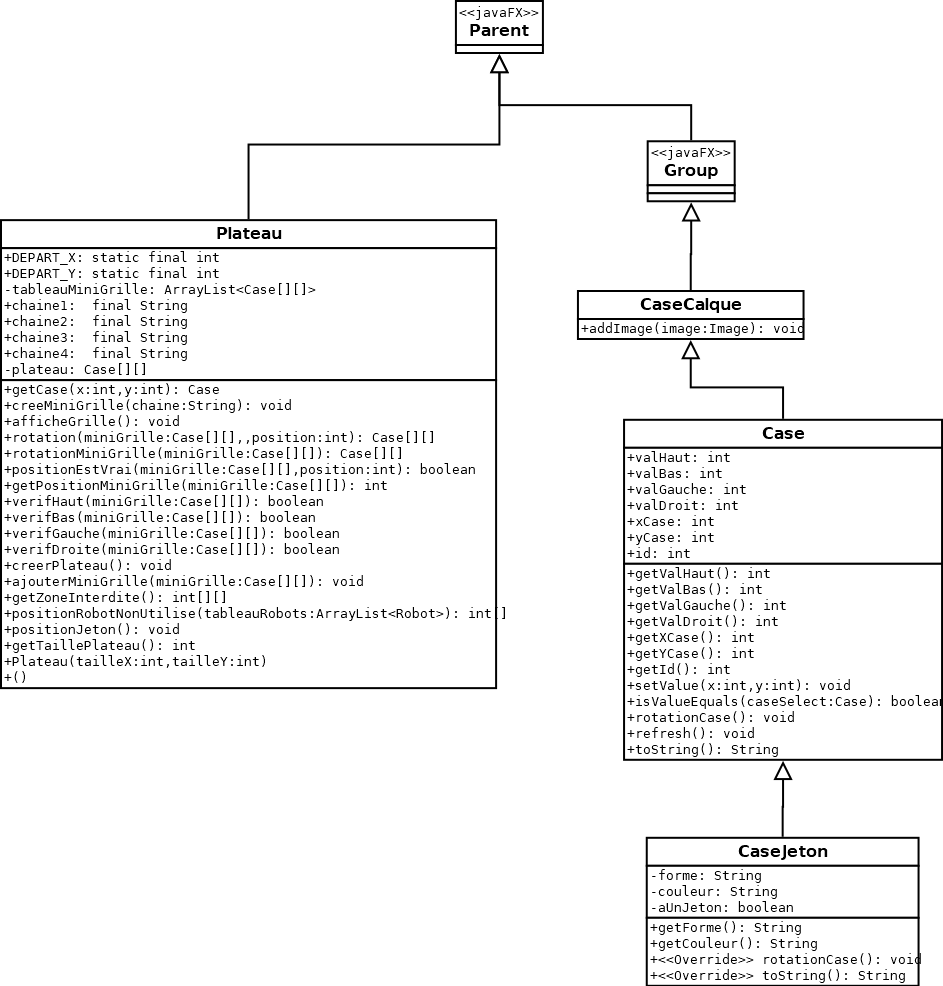
\includegraphics[scale=0.45]{images/diagrammePlateau.png}
                \caption{Diagramme du package plateau}
            \end{figure}
            
            
 %%%%%%%%%%%%%%%%%%%%%%%%%%%%%%%%%%%%%%%%%%%%%%%%%%%%%%%%%%%%%%%%%%%%%%%%%%%%%%%%%%%%%%%%%%%%%%%%%%%%%%%%%%%%%%%%%%%%%%%%

\section{Développement du jeu}
    \subsection{Création du plateau}
        \subsubsection{Création des mini-plateaux}
            Pour concevoir le Ricochet Robot, la première question que nous nous sommes posés à été: "comment devons-nous créer le plateau?". Le plateau du Ricochet Robots est un ensemble de "mini-plateaux" qui, une fois assemblés, forment ce plateau. Dans la version du jeu de société, il existe quatre morceaux de plateaux, chaque morceau ayant deux faces. Dans notre version, nous avons voulu garder que quatre faces, une pour chaque morceau, qui étaient suffisantes pour la réalisation du Ricochet Robot.
            
            \begin{figure}[H]
            	\centering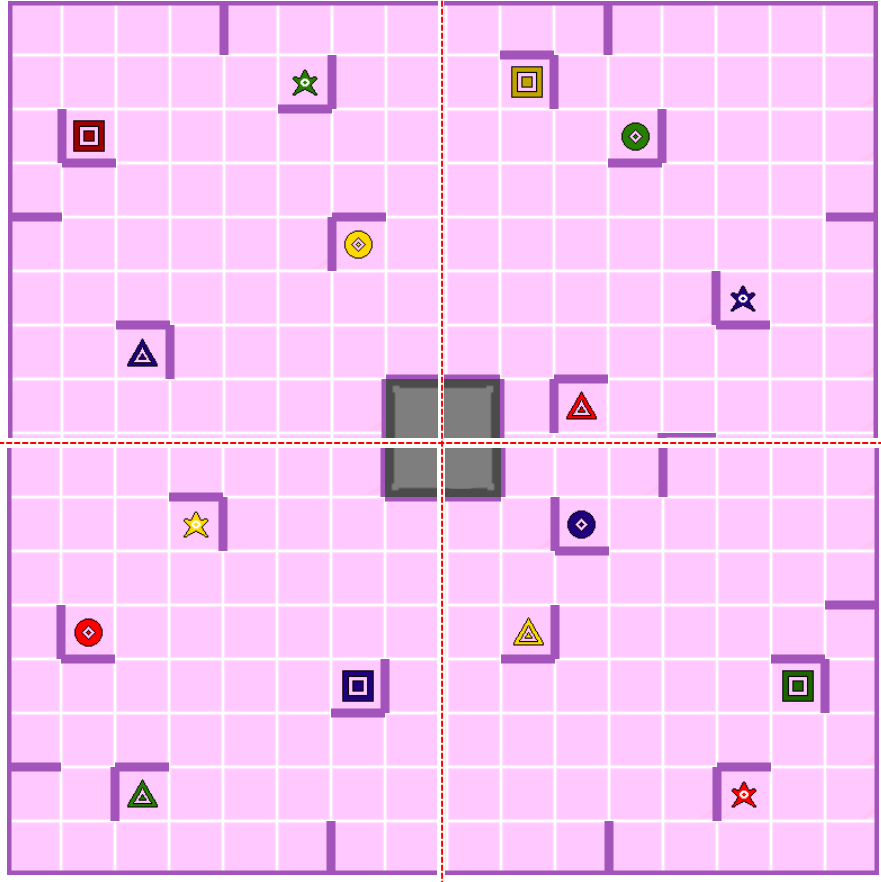
\includegraphics[width=0.5\textwidth]{images/plateauDecoupe.png}
            	\caption{Composition du plateau}
            \end{figure}
            
            Pour créer le plateau, nous devions commencer par la création de ces mini-plateaux. Ces quatre mini-plateaux ont été chacun, représentés par des tableaux en deux dimensions, contenant des cases et des murs. 
            
            C'est à ce moment là que nous devions réfléchir sur la représentation de ces cases et de ces murs. Après observation du plateau, nous avons remarqué que ce plateau était composé que de onze cases différentes.
            
            \begin{figure}[H]
            	\centering
\includegraphics[scale=0.60]{images/liste_cases.png}
            	\caption{Ensemble des cases existantes}
            \end{figure}
            
            Ces cases ont toutes un élément en commun: la possibilité d'avoir un mur en haut, en bas, à gauche, ou à droite.
    
            \vspace{0.5cm}
            \begin{center}
                \begin{tikzpicture}
                    \draw (1,1) rectangle (5,5);
                    \draw[color=red] (1,1.5) -- (5,1.5);
                    \draw[color=green] (1,4.5) -- (5,4.5);
                    \draw[color=blue] (1.5,1) -- (1.5,5);
                    \draw[color=olive] (4.5,5) -- (4.5,1);
                    \node[color=red] (pos) at (3,0.5) {BAS};
                    \node[color=green] (pos) at (3,5.5) {HAUT};
                    \node[color=blue] (pos) at (0,3) {DROIT};
                    \node[color=olive] (pos) at (6,3) {GAUCHE};
                    
                    \node (posi) at (10,5) {[ HAUT, DROIT, BAS, GAUCHE ]};
                    \draw[->] (5,4) -- (posi);
                \end{tikzpicture}
            \end{center}  
            \vspace{0.5cm}
            
            Nous avons donc décidé de représenter chaque case de cette manière: la présence d'un mur en haut entraînait un 1 à la valeur de HAUT, la présence d'un mur en haut entraînait un 1 à la valeur de DROIT, et ainsi de suite pour les autres côtés. Ce qui donne par exemple:
            
            \vspace{0.5cm}
            
            \begin{figure}[H]
                \centering
                \begin{tikzpicture}
                    \draw[fill=red] (0,2) rectangle (2, 1.75);
                    \draw (0,0) rectangle (2,2);
                    \draw[dotted] (0,0.25) -- (2,0.25);
                    \draw[dotted] (0,1.75) -- (2,1.75);
                    \draw[dotted] (0.25,0) -- (0.25,2);
                    \draw[dotted] (1.75,0) -- (1.75,2);
                    
                    \node (bool) at (6,1) {[ True, False, False, False ]};
                    \node (bin) at (10,1) {[1,0,0,0]};
                    \draw[->] (bool) -- (bin);
                \end{tikzpicture}
                \caption{Cas de figure pour un mur en haut de la case}
            \end{figure}
            
    
            Pour ne pas alourdir chaque mini-plateau en créant un tableau à trois dimension (un tableau en deux dimensions dont chaque élément contient elle-même un tableau), nous avons donc créé une classe Case, contenant quatre variables nommées "valHaut, valBas, valGauche et valDroite" qui remplace le format de tableau [HAUT, DROIT, BAS, GAUCHE]. Nous avons alors avec un tableau à deux dimension dont chaque élément contient une instance de Case.
            
            Á ce moment là, il fallait donc créer les quatre mini-tableaux. La position de chaque case de chaque mini-tableau est importante et inchangeable, car les modèles des mini-plateaux du jeu de société sont réalisés de manière à avoir une solution à toute situation de jeu. Nous avons donc gardé les modèles existants. 
            
            Nous avons donc cherché une manière de sauvegarder ces quatre modèles de mini-plateau dans le code, et ainsi qu'a partir ce cette sauvegarde, les mini-plateaux se créent. 
            
            Nous avons opté pour un modèle suivant:
            \vspace{0.5cm}
            \lstinputlisting[language=Java]{code/var.java}
    
            
            Cette manière de faire permettait qu'a partir d'une suite de nombres, le programme créé un mini-plateau. Le code correspondant est le suivant:
                
            \begin{algorithm}[H]%-------------------------------------------
                \DontPrintSemicolon
                \KwIn{Une chaine de caractère représentant le mini-plateau}
                \KwOut{Le mini-plateau}
                $tableauDeChiffre \gets chaineDeCaractere.split(",")$
                $tailleTableau \gets \sqrt{tableauDeChiffre.length()}$
                $index \gets 0$
                $miniGrille[][] \gets {nouvelle \ instance \ de \ Case }$
                \For{$y \gets 0$ \textbf{à} $tailleTableau$}{
                  \For{$x \gets 0$ \textbf{à} $tailleTableau$}{
                    $miniGrille[x][y] \gets new \ Case(Utilitaire.intToBinary(tab1D[index]), x, y)$
                    $index++$
                    }
                 }
                \Return{$miniGrille$}\;
                \caption{\sc Création d'un mini-plateau}
            \end{algorithm}%-------------------------------------------
            
            Chaque nombre correspond à un type de case. Le numéro n'est pas pris au hasard: en reprenant la figure 8 ci-dessus, nous avons vu que une case ayant un mur en haut correspondait à [1,0,0,0]. L'idée était de récupérer ces chiffres, formant "1000", qui en nombre binaire est un "8". Une case avec un mur en haut correspond donc au chiffre "8". Le système est le même pour chaque case.
            
            \subsubsection{Positionnement des mini-plateaux}
    
            Comme le plateau est composé de quatre parties, chaque mini plateau ont quatre possibilités de positionnement afin de former le plateau final.
        
            \begin{center}
                \begin{tikzpicture}
                    \draw (0,0) rectangle (4,4);
                    \draw[dotted] (0,2) -- (4,2);
                    \draw[dotted] (2,0) -- (2,4);
                    \node (4) at (1,1) {4};
                    \node (3) at (3,1) {3};
                    \node (2) at (3,3) {2};
                    \node (1) at (1,3) {1};
                \end{tikzpicture}
            \end{center}
            
            Pour les positionner de manière aléatoire, nous avons fait en sorte que le programme tire une position pour chaque mini-plateau. Cependant ce n'est pas suffisant, puisqu'il faut que les murs de chaque mini-plateau soient bien positionnés, sinon nous nous retrouverions avec des plateaux de cette forme:
            
            \begin{figure}[H]
                \centering
                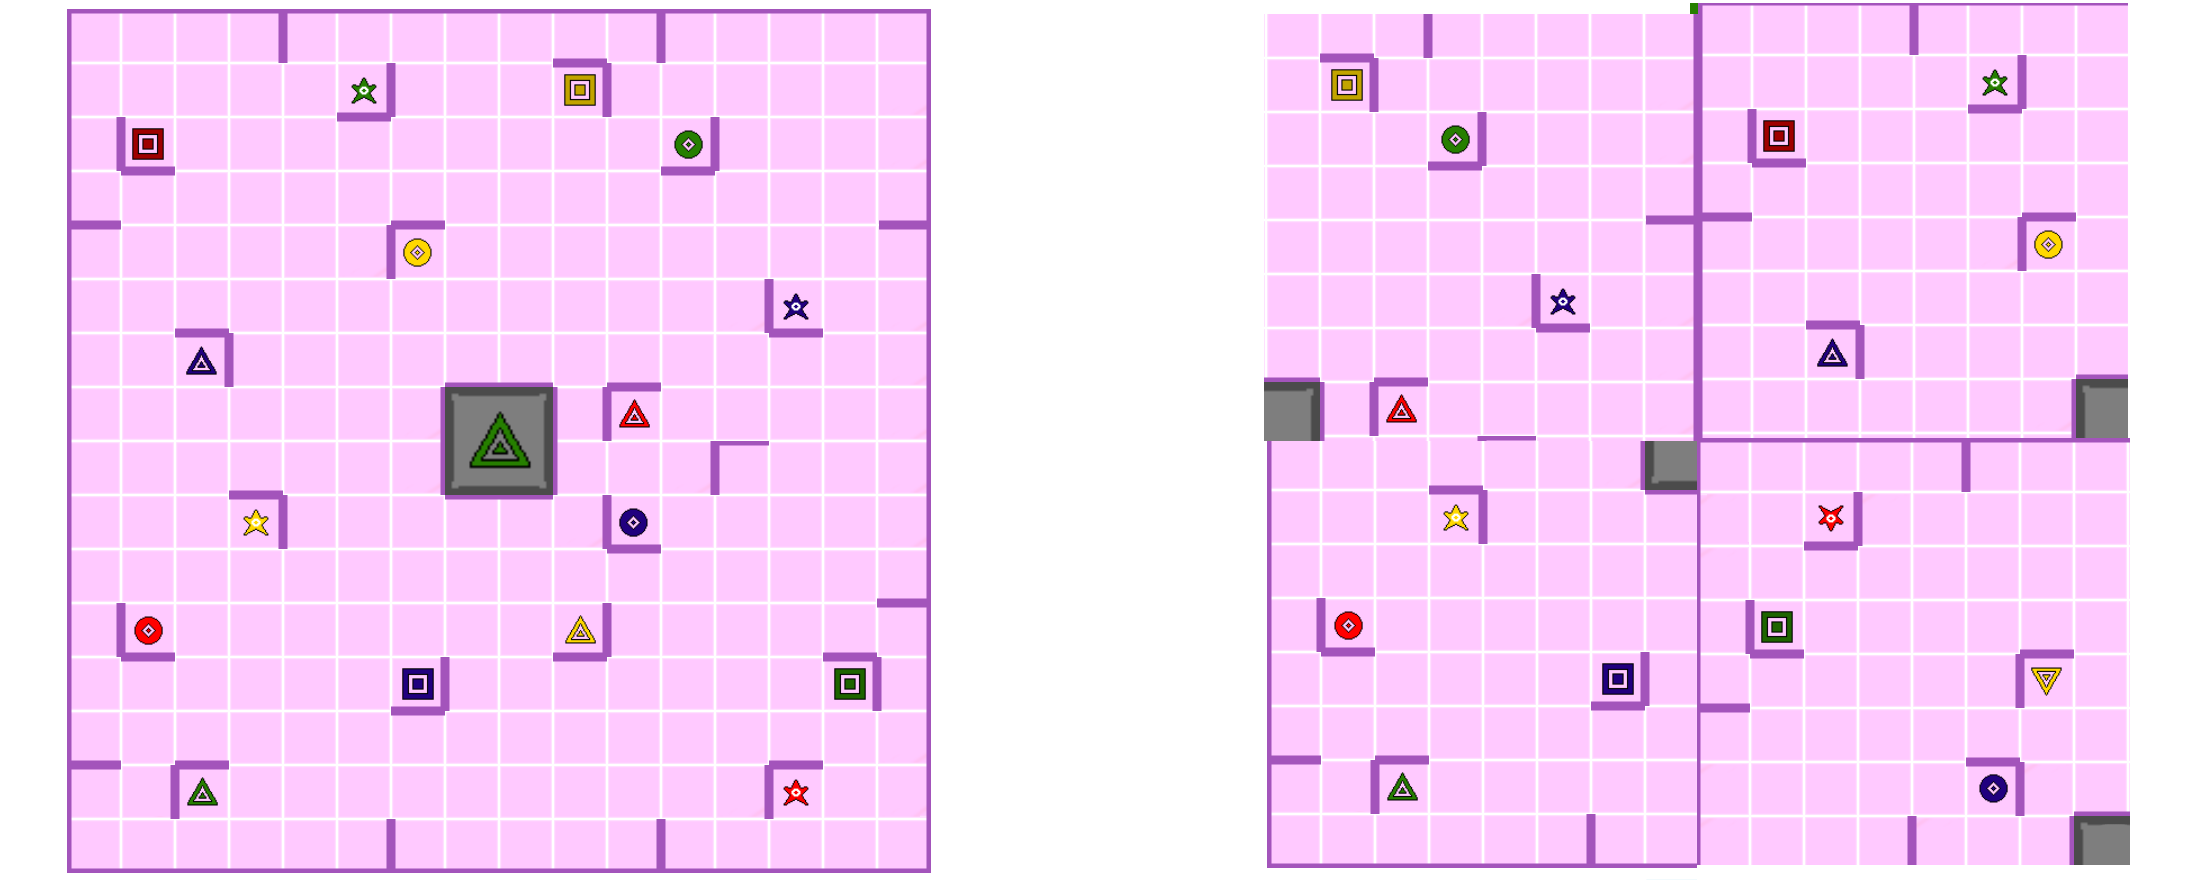
\includegraphics[scale=0.2]{images/bonvsmauvais.png}
                \caption{Bon (à gauche) et mauvais plateau (à droite)}
            \end{figure}
            
            Pour cela, il faut vérifier l'emplacement des murs qui composent les bordures, et affecter une rotation à ces mini-plateaux tant que le mini-plateau n'est pas valide apr rapport à sa position:
            
            \begin{algorithm}[H]%-------------------------------------------
                \DontPrintSemicolon
                \KwIn{le mini-plateau, la position affectée au mini-plateau}
                \KwOut{Le mini-plateau}
                $miniGrilleRota \gets new \ Case(miniGrille.length(), miniGrille.length())$
                \For{$y \gets 0$ \textbf{à} $miniGrille.length()$}{
                  \For{$x \gets 0$ \textbf{à} $miniGrille.length()$}{
                        $miniGrilleRota[x][y] \gets miniGrilleRota[x][y]$
                    }
                 }
                 \While{positionEstVraie(miniGrilleRota, position) != true}{
                    $miniGrilleRota[x][y] \gets rotationMiniGrille(miniGrilleRota)$
                 }
                \Return{$miniGrilleRota$}\;
                \caption{\sc Rotation d'un mini-plateau}
                Avec positionEstVrai(), une méthode qui permet de vérifier les murs des bordures
            \end{algorithm}%-------------------------------------------
        
            \begin{algorithm}[H]%-------------------------------------------
                \DontPrintSemicolon
                % \SetKwData{JeuNonTrie}{jeuNonTrie}
                % \SetKwData{JeuTrie}{jeuTrie}
                \KwIn{un mini-plateau}
                \KwOut{Le mini-plateau dans une rotation de 90 degrés}
                $miniGrilleRota \gets new \ Case(miniGrille.length(), miniGrille.length())$
                \For{$y \gets 0$ \textbf{à} $miniGrille.length()$}{
                  \For{$x \gets 0$ \textbf{à} $miniGrille.length()$}{
                        $miniGrilleRota[x][y] \gets miniGrilleRota[y][miniGrille.length - x - 1]$
                        $miniGrilleRota[x][y].rotationCase()$
                    }
                 }
                 \While{positionEstVraie(miniGrilleRota, position) != true}{
                    $miniGrilleRota[x][y] \gets rotationMiniGrille(miniGrilleRota)$
                 }
                \Return{$miniGrilleRota$}\;
                \caption{\sc Rotation du mini-plateu de 90 degrés}
            \end{algorithm}%-------------------------------------------
        
            \newpage
            La méthode rotationCase consiste à décaler d'un cran les valeurs de la classe Case selon le modèle suivant:
            
           \begin{figure}[H]
               \centering
               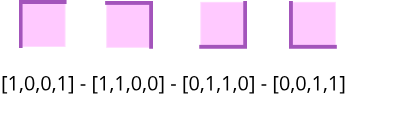
\includegraphics[scale=0.7]{images/rotaCase.png}
           \end{figure}
           
           Le code est le suivant:
           
            \lstinputlisting[language=Java]{code/rotaCase.java}
            
                
        \subsubsection{Création du plateau}
            Une fois que chaque mini-plateau était bien positionné, c'est à ce moment là que nous devions créer le plateau. Pour cela, nous avons crée un tableau à deux dimensions de Case, représentant le plateau et chaque coin de ce plateau est parcouru pour y affecter les valeurs contenues dans chaque mini-plateau. L'algorithme utilisé est le suivant:
            \newpage
      
            \begin{algorithm}[H]%-------------------------------------------
                \DontPrintSemicolon
                \KwIn{Le mini-plateau à placer}
                $ plateau[][] \gets nouvelle \ instance \ de \ Case $
                $ demiTabX \gets divise \ le \ tableau \ en \ largeur \ par \ 2$
	        	$ demiTabY \gets divise \ le \ tableau \ en \ hauteur \ par \ 2$
                
                \If{la position du mini-plateau doit être à 1}{
                    \For{$y \gets 0$ \textbf{à} $demiTabY$}{
                        \For{$x \gets 0$ \textbf{à} $demiTabX$}{
                            $plateau[x][y] \gets miniPlateau[x][y]$
                        }
                    }
                }
                \uElseIf{la position du mini-plateau doit être à 2}{
                    \For{$y \gets 0$ \textbf{à} $demiTabY$}{
                        \For{$x \gets demiTabX$ \textbf{à} $tableau.length$}{
                            $plateau[x][y] \gets miniPlateau[x-demiTabX][y]$
                        }
                    }
                }
                \uElseIf{la position du mini-plateau doit être à 3}{
                    \For{$y \gets demiTabY$ \textbf{à} $tableau.length$}{
                        \For{$x \gets demiTabX$ \textbf{à} $tableau.length$}{
                            $plateau[x][y] \gets miniPlateau[x-demiTabX][y-demiTabY]$
                        }
                    }
                }
                \uElseIf{la position du mini-plateau doit être à 4}{
                    \For{$y \gets demiTabY$ \textbf{à} $tableau.length$}{
                        \For{$x \gets 0$ \textbf{à} $demiTabX$}{
                            $plateau[x][y] \gets miniPlateau[x][y-demiTabX]$
                        }
                    }
                }
                
                \caption{\sc Création du plateau}
            \end{algorithm}%-------------------------------------------
    
    \subsection{Positionnement des robots}
        Lors du lancement du jeu, les robots ne pouvaient pas être positionnés sur n'importe quelle case. Certaines cases étaient dites "interdites". Il s'agissait des cases où se situait les jetons, ainsi que la partie du milieu, comme montré ci-dessous:
        
        \begin{figure}[H]
            \centering
            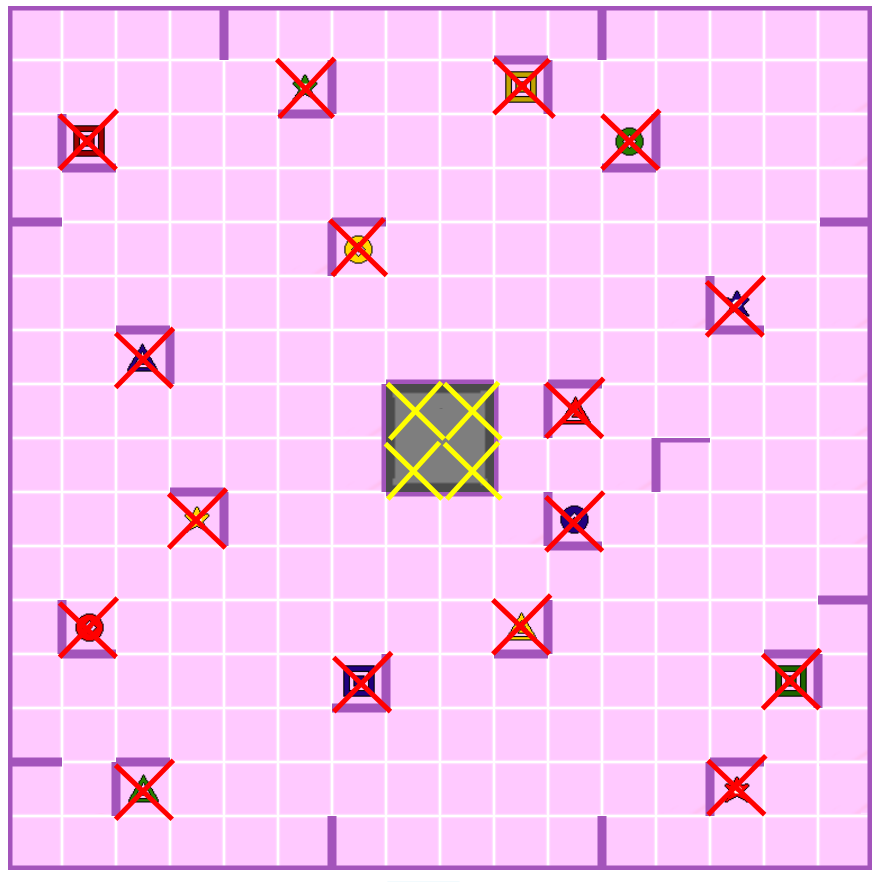
\includegraphics[scale=0.17]{images/positionInterdite.png}
            \caption{Positions initiales interdites au lancement du jeu pour les robots}
        \end{figure}
        
        Bien évidement, deux robots ne pouvaient pas être sur la même case. Il fallait donc également vérifier qu'à chaque nouveau robot créé, les cases utilisées par les autres robots, ne soient plus disponible pour ce nouveau robot.
        
        Étant donné que les positions interdites étaient qu'une minorité, il était plus judicieux de d'abord tirer une position de manière aléatoire, c'est-à-dire un nombre représentant la position en X du robot, et un autre pour la position Y. Á partir de ces deux nombres, il fallait ensuite vérifier si la coordonnée correspondante n'était pas similaire à une case interdite ou une position précédemment donné a un robot. Dans le cas où la coordonné tirée n'était pas valide, le processus recommençait tant que celle-ci n'était pas satisfaisante. 
        
        L'algorithme correspondant à la position des robots est la suivante:
        
        \begin{algorithm}[H]%-------------------------------------------
            \DontPrintSemicolon
            \KwOut{Les coordonnées correctes pour le robot}
            $surJeton \gets false$
            $surRobot \gets false$
            $surCaseInterdite \gets false$
            \Do{$surJeton \ or \ surCaseInterdite \ or \ surRobot$}{
                $aleaX \gets tirage \ d'un \  nombre \  aléatoire \  entre \  0 \  et \  15$
                $aleaY \gets tirage \ d'un \  nombre \  aléatoire \  entre \  0 \  et \  15$
                \If{surJeton}{
                    $continue$
                }
                $surCaseInterdite = estSurCaseInterdite()$
                \If{$surCaseInterdite$}{
				    $continue$
			    }
    			\If{$robotsExistants! \gets \emptyset$}{
    				$surRobot \gets estSurAutresRobots(aleaX,aleaY)$
    
    				\If{$surRobot$}{
    					$continue$
    				}
                }
                $position[] \gets {aleaX, aleaY}$
            }
            \Return{$position[]$}
            \caption{\sc Positionnement des robots à l'état initial}
        \end{algorithm}%-------------------------------------------
        
    \subsection{Déplacements et collisions des robots}
    
        Lorsque l'on veut déplacer un robot vers une direction, ce robot se déplace dans cette direction, qu'en ligne droite jusqu'à ce qu'il rencontre un obstacle. L'obstacle peut être un mur ou alors un autre robot. Pour que le robot s'arrête à un obstacle, il fallait mettre en place un système de collision. 
        
        
         \begin{figure}[H]
            \centering
            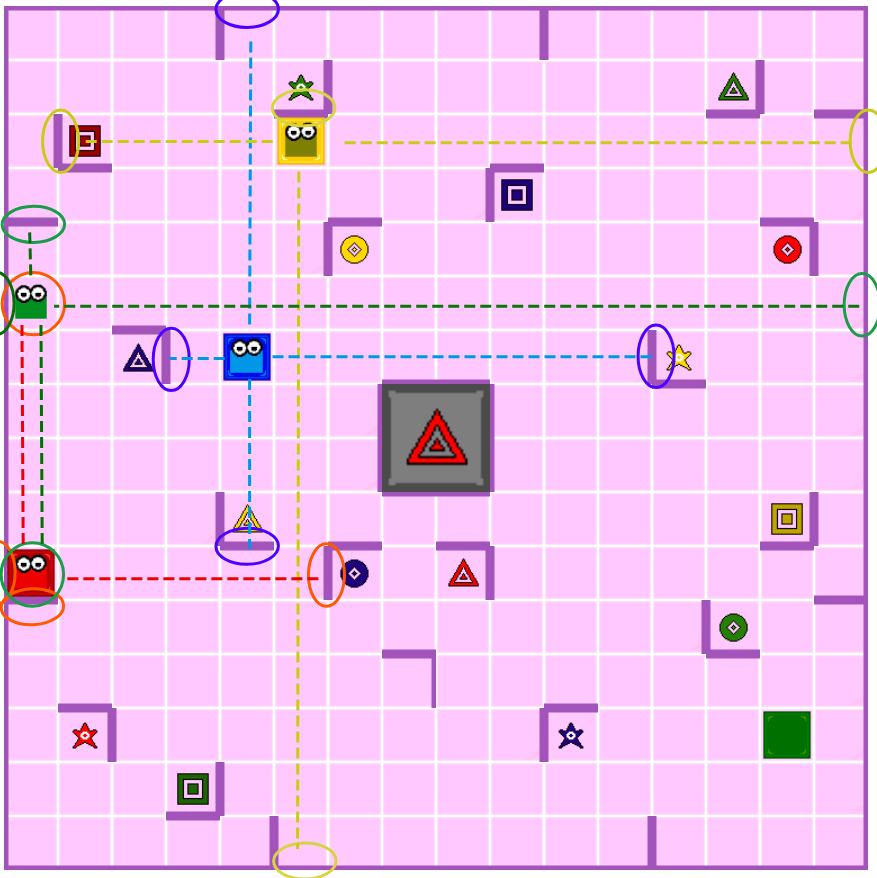
\includegraphics[scale=0.25]{images/collision.png}
            \caption{Ensemble de collisions pour chaque déplacement des robots à un état donné}
        \end{figure}
        
        Pour pouvoir mettre en place ce système de collision lors d'un déplacement, il a donc fallu faire en sorte de vérifier la case actuelle du robot à déplacer, si elle contenait un mur sur son chemin et si la case suivante contenait un mur sur son chemin ou un autre robot.
        
        \begin{figure}[H]
            \centering
            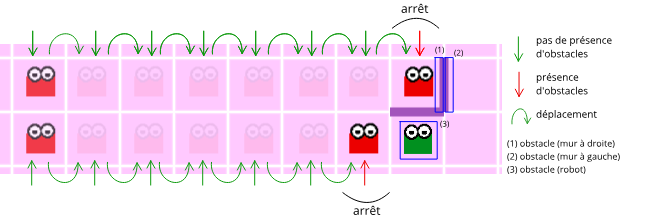
\includegraphics[scale=0.7]{images/deplacements.png}
            \caption{Vérifications du robot lors du déplacement}
        \end{figure}
        
        \l'algorithme correspondant à ces vérification est le suivant:
        
        \begin{algorithm}[H]%-------------------------------------------
            \DontPrintSemicolon
            \KwIn{La direction de déplacement}
    		\If{$direction == haut$}{
    			\While{$pas\ de \ mur\ en\ haut\ de\ la\ case\ actuelle$ \textbf{et} $pas\ de\ 
    			mur\ en\ bas de\ la\ case\ suivante $ \textbf{et}  $  !estUneCollisionRobot(direction, robot)$}{
    				$deplacement\ d'une\ case\ vers\ le\ haut$
    			}
    		}
    		\uElseIf{$direction == bas$}{
    			
    			\While{$pas\ de \ mur\ en\ bas\ de\ la\ case\ actuelle$ \textbf{et} $pas\ de\ 
    			mur\ en\ haut\ de\ la\ case\ suivante $ \textbf{et}  $  !estUneCollisionRobot(direction, robot)$}{
    				$deplacement\ d'une\ case\ vers\ le\ bas$
    			}
    		}
    		\uElseIf{$direction == gauche$}{
    			\While{$pas\ de \ mur\ a\ gauche\ de\ la\ case\ actuelle$ \textbf{et} $pas\ de\ 
    			mur\ a\ droite\ de\ la\ case\ suivante $ \textbf{et}  $  !estUneCollisionRobot(direction, robot)$}{
    				$deplacement\ d'une\ case\ vers\ la\ gauche$
    			}
    		}
    		\uElseIf{$direction == droite$}{
    			 \While{$pas\ de \ mur\ a\ droite\ de\ la\ case\ actuelle$ \textbf{et} $pas\ de\ 
    			mur\ a\ gauche\ de\ la\ case\ suivante $ \textbf{et}  $  !estUneCollisionRobot(direction, robot)$}{
    				$deplacement\ d'une\ case\ vers\ la\ droite$
    			}
    		}
            \caption{\sc Déplacement d'un robot jusqu'à collision}
        \end{algorithm}%-------------------------------------------
     
    \subsection{Sélection des robots}
        %****************** selection robots **************************%
       
        
            Pendant une partie, il est souvent nécessaire de déplacer les autres robots afin qu'ils fassent office d'obstacles, ce qui peut permettre de récupérer au robot devant jouer (celui qui doit aller sur la case correspondante) de récupérer le jeton avec moins de mouvements qu'en temps normal.
            \paragraph{}
            Pour cela, nous voulions faire en sorte qu'au moment où le joueur clique sur un autre robot, c'est ce nouveau robot qui à la possibilité de se déplacer, et si le joueur clique ailleurs sur le plateau (en l'occurrence sur une case du plateau), ou sur le robot qui doit attraper le jeton, c'est de nouveau le robot devant jouer qui peut se déplacer.
            \paragraph{}
            Pour mettre en place ce système, nous avons donc mis en place le design pattern \textit{Observer}. Ce design pattern permet dans notre projet de gérer des événements souris sur un robot et une case. Dans notre projet, nous avons la classe State qui est à la fois l'observeur de l'événement sur un robot et l'observeur de l'événement sur une case. D'un autre côté, la classe Case et la classe Robot représente les observables. Le pattern observer est mis en place de la manière suivante:
            
           \begin{figure}[H]
                \centering
                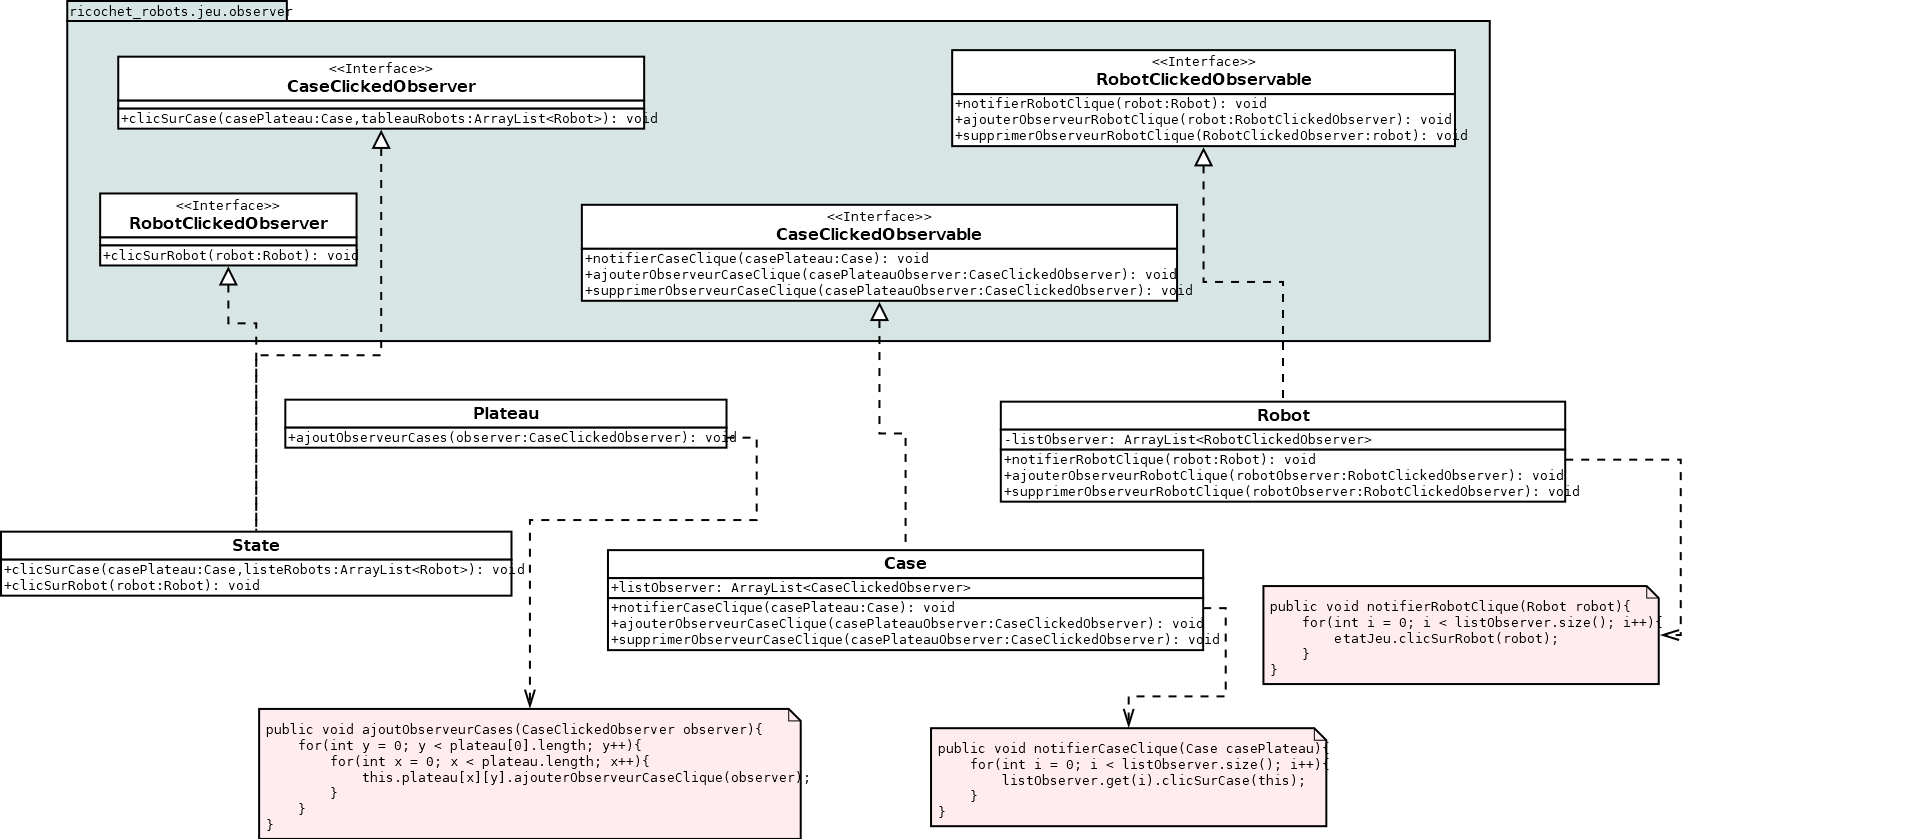
\includegraphics[scale=0.25]{images/patternObserverRobot.png}
                \caption{Diagramme de l'implémentation du pattern observer}
            \end{figure}
            
            Lors de la création de chaque robot, nous ajoutons à chaque robot, la classe State comme observeur de chaque robot. Dans la classe Plateau, nous réalisons la même chose sur chacune des cases (en ajoutant la classe State comme observer). Dans la classe State, nous avons également les méthodes redéfinies des interfaces CaseClickedObserveret RobotClickedObserver, c'est-à-dire la méthode clicSurCase(Case case) et la méthode clicSurRobot(Robot robot). Cest deux méthodes contiennent l'action réalisée lors du clic sur l'un de ces objets. Dans les classes Robot et Classe, nous avons une méthode qui est redéfini des interfaces RobotClickedObservable (pour la classe Robot) et CaseClickedObservable  (pour la classe Case). Ces méthodes sont appelés lorsque le robot (ou la case) est cliquée. Cela permet de prévenir les observeurs du clic réalisé sur l'objet (en l'occurrence ici nous avons que la classe State qui est observeur). Plus précisément, la méthode notifierRobotClique appelle directement la méthode clicSurRobot() pusqu'elle à accès à la classe State, et la la méthode notifierCaseClique() va récupérer dans son Arraylist d'observeurs, les différents observeurs et va appeler la méthode clicSurCase() de chaque observateur, donc la classe State.
            
            Le contenu de la méthode clicSurRobot() est le suivant: 
            \lstinputlisting[language=Java]{code/clicRobot.java}
            Cela permet de changer le robot actuel, car au déplacement d'un robot, le déplacement se fait par défaut en fonction du de la variable contenue dans robotActuel. 
            
            Le contenu de la méthode clicSurCase() est le suivant:
            \lstinputlisting[language=Java]{code/clicCase.java}
            Cet appel à la méthode robotAJouer() permet de rechercher le robot qui doit atteindre l'objectif parmi tout les robots existants. Une fois le robot trouvé, ce robot est affecté à la variable robotActuel, et donc le joueur récupérait le contrôle du robot devant jouer.   
            

        
Quand l'état de la classe change elle doit envoyer un signal a tout ses observateurs qui doivent effectuer l'action nécessaire en fonction du nouvel état de la classe.
         

\newpage %%%%%%%%%%%%%%%%%%%%%%%%%%%%%%%%%%%%%%%%%%%%%%%%%%%%%%%%%%%%%%%%%%%%%%%%%%%%%%%%%%%%%%%%%%%%%%%%%%%%%%%%%%%%%%%%%%%%%%%%

\section{Implémentation de l'algorithme}
    \subsection{Algorithme de parcours en largeur (BFS)}
        \subsubsection{Principe}
            D'après Wikipédia\cite{bfs}, l'algorithme de parcours en largeur ou BFS, pour Breadth First Search en anglais est un algorithme permettant le parcours d'un graphe ou d'un arbre étage par étage. L'idée est de comencer par explorer un nœud parent, puis l'ensemble de ces successeurs, puis les successeurs non explorés de ces successeurs, et ainsi de suite jusqu'a trouver une solution. 
            
            Il s'agit d'un algorithme très utile, à la fois pour la recherche de chemin, mais aussi pour certains types d'analyse de carte avec notamment l'analyse des cartes de distance.
            \begin{figure}[H]
        
                \begin{tikzpicture}[scale=0.75]
                    \node[fill=orange,draw=black,text=black, shape=circle] (S0) at (3,4) {S0};
                    \node[fill=pink,draw=black,text=black, shape=circle] (S1) at (1,2) {S1};
                    \node[fill=pink,draw=black,text=black, shape=circle] (S2) at (5,2) {S2};
                    \node[draw=black,text=black, shape=circle] (S3) at (0,0) {S3};
                    \node[draw=black,text=black, shape=circle] (S4) at (2,0) {S4};
                    \node[draw=black,text=black, shape=circle] (S5) at (4,0) {S5};
                    \node[draw=black,text=black, shape=circle] (S6) at (6,0) {S6};
                    
                    \draw[<-] (S0) -- (S1);
                    \draw[<-] (S1) -- (S3);
                    \draw[<-] (S1) -- (S4);
                    \draw[<-] (S0) -- (S2);
                    \draw[<-] (S2) -- (S5);
                    \draw[<-] (S2) -- (S6);
                \end{tikzpicture}
                \begin{tikzpicture}[scale=0.75]
                    \node[fill=green,draw=black,text=black, shape=circle] (S0) at (3,4) {S0};
                    \node[fill=orange,draw=black,text=black, shape=circle] (S1) at (1,2) {S1};
                    \node[fill=pink,draw=black,text=black, shape=circle] (S2) at (5,2) {S2};
                    \node[fill=pink,draw=black,text=black, shape=circle] (S3) at (0,0) {S3};
                    \node[fill=pink,draw=black,text=black, shape=circle] (S4) at (2,0) {S4};
                    \node[draw=black,text=black, shape=circle] (S5) at (4,0) {S5};
                    \node[draw=black,text=black, shape=circle] (S6) at (6,0) {S6};
                    
                    \draw[<-] (S0) -- (S1);
                    \draw[<-] (S1) -- (S3);
                    \draw[<-] (S1) -- (S4);
                    \draw[<-] (S0) -- (S2);
                    \draw[<-] (S2) -- (S5);
                    \draw[<-] (S2) -- (S6);
                 \end{tikzpicture}
                 \begin{tikzpicture}[scale=0.75]
                    \node[fill=green,draw=black,text=black, shape=circle] (S0) at (3,4) {S0};
                    \node[fill=green,draw=black,text=black, shape=circle] (S1) at (1,2) {S1};
                    \node[fill=orange,draw=black,text=black, shape=circle] (S2) at (5,2) {S2};
                    \node[fill=pink,draw=black,text=black, shape=circle] (S3) at (0,0) {S3};
                    \node[fill=pink,draw=black,text=black, shape=circle] (S4) at (2,0) {S4};
                    \node[fill=pink,draw=black,text=black, shape=circle] (S5) at (4,0) {S5};
                    \node[fill=pink,draw=black,text=black, shape=circle] (S6) at (6,0) {S6};
                    
                    \draw[<-] (S0) -- (S1);
                    \draw[<-] (S1) -- (S3);
                    \draw[<-] (S1) -- (S4);
                    \draw[<-] (S0) -- (S2);
                    \draw[<-] (S2) -- (S5);
                    \draw[<-] (S2) -- (S6);
                 \end{tikzpicture}
                 
                \begin{tikzpicture}[scale=0.75]
                    \node[fill=green,draw=black,text=black, shape=circle] (S0) at (3,4) {S0};
                    \node[fill=green,draw=black,text=black, shape=circle] (S1) at (1,2) {S1};
                    \node[fill=green,draw=black,text=black, shape=circle] (S2) at (5,2) {S2};
                    \node[fill=orange,draw=black,text=black, shape=circle] (S3) at (0,0) {S3};
                    \node[fill=pink,draw=black,text=black, shape=circle] (S4) at (2,0) {S4};
                    \node[fill=pink,draw=black,text=black, shape=circle] (S5) at (4,0) {S5};
                    \node[fill=pink,draw=black,text=black, shape=circle] (S6) at (6,0) {S6};
                    
                    \draw[<-] (S0) -- (S1);
                    \draw[<-] (S1) -- (S3);
                    \draw[<-] (S1) -- (S4);
                    \draw[<-] (S0) -- (S2);
                    \draw[<-] (S2) -- (S5);
                    \draw[<-] (S2) -- (S6);
                \end{tikzpicture}
                  \hspace{3cm}
                \begin{tikzpicture}
                    \draw[dotted] (0,0) rectangle (8,3.5);
                    \draw[fill=green] (1,2.75) circle (0.25);
                    \draw[fill=orange] (1,2) circle (0.25);
                    \draw[fill=pink] (1,1.25) circle (0.25);
                    \draw (1,0.5) circle (0.25);
                    
                    
                    \node (dE) at (3,2.75) {noeud exploré};
                    \node (ecE) at (4.35,2) {noeud en cours d'exploration};
                    \node (ecE) at (4.05,1.25) {noeud connu, non exploré};
                    \node (nE) at (3.05,0.5) {noeud inconnu};
                \end{tikzpicture}
            \end{figure}
            
        \subsubsection{Implémentation dans le Ricochet Robots}
            Dans le cas du Ricochet Robots, un noeud est représenté par un état du jeu et la flèche par un déplacement d'un robot. Lorsque un robot réalise un déplacement, si ce robot ne reste pas sur la même case, un nouvel état de jeu est donc crée. Dès lors que l'on trouve un état gagnant, l'algorithme doit s'arrêter puisque le chemin vers ce noeud sera forcément le chemin le plus court avec son exploration étage par étage.
            
          \begin{figure}[H]
                \centering
                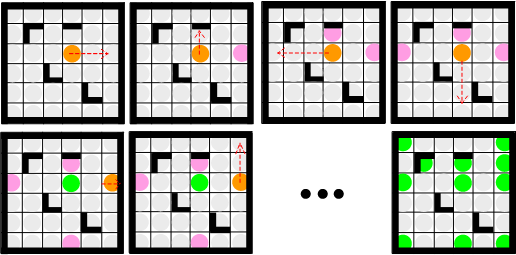
\includegraphics[scale=0.85]{images/bfsRicochet.png}
                \caption{Visualisation de l'algorithme BFS sur le Ricochet Robots pour un robot}
            \end{figure}
             
            
            Bien que cet algorithme fonctionne, il s'agit d'un algorithme qui met un certain temps pour résoudre le problème puisque le nombre de mouvements est souvent supérieure à 4 (observations faîtes durant les nombreuses simulations réalisées). Il faut donc pour cela trouver des méthodes d'optimisation.
       
            \begin{figure}[H]
                \centering
                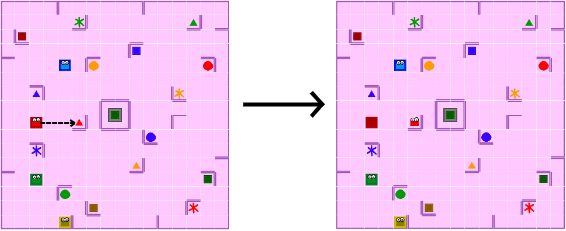
\includegraphics[scale=0.75]{images/stateToState.png}
                \caption{État A vers un nouvel état B après déplacement}
            \end{figure}
    \subsection{Optimisation}
        L'algorithme A* est un algorithme regroupant l'algorithme BFS et l'ajout d'une heuristique. Cette heuristique permet d'aller plus rapidement vers la solution, et ainsi permet d'éviter d'explorer des noeuds "inutiles".
        Parmi les heuristiques existants, le plus connu est celui du "vol d'oiseau". Cet heuristique permet de prioriser certains déplacements. Par exemple dans l'image ci-dessous, dans un déplacement d'une case par une case, les mouvements prorisées seront les déplacements vers le haut et la gauche.
        
           \begin{figure}[H]
                \centering
                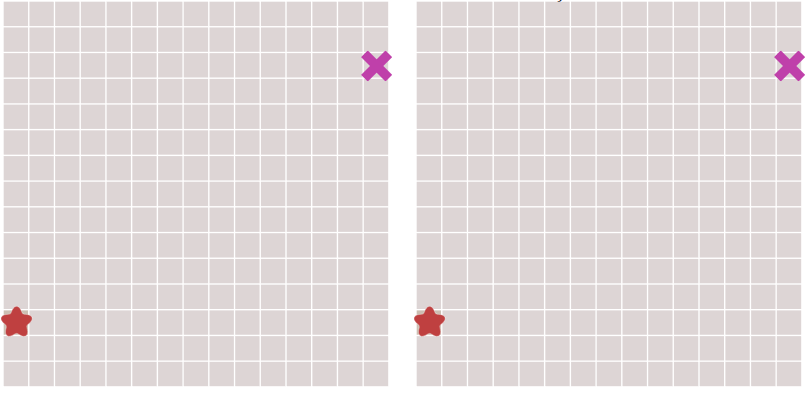
\includegraphics[scale=0.75]{images/1.png}
                \caption{image\cite{redblob} avec et sans heuristique à l'état initial}
            \end{figure}
        
        Cet heuristique permet une réelle optimisation. Nous pouvons ainsi le voir sur cette image l'importance de l'heuristique.
        
           \begin{figure}[H]
                \centering
                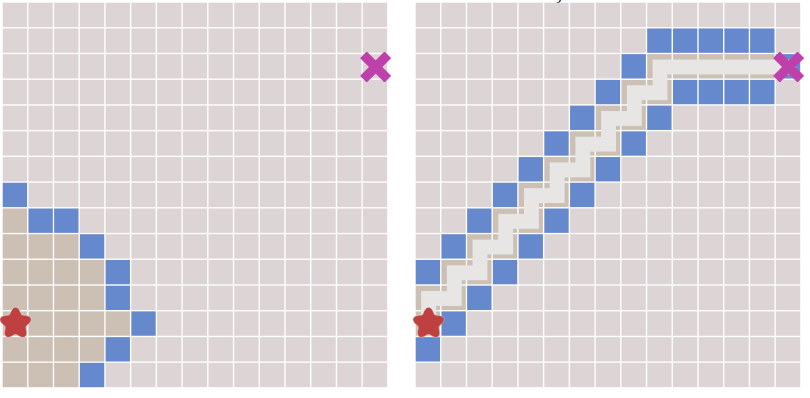
\includegraphics[scale=0.75]{images/2.png}
                \caption{image\cite{redblob} sans et avec heuristique après 23 noeuds explorés }
            \end{figure}
        
    Ainsi, pour connaître l'ensemble des états possibles d'une partie, le but était de déplacer chaque robot, dans chaque direction, et de sauvegarder chaque nouvel état. Lorsque qu'il y avait deux états similaires, c'est-à-dire lorsque les quatre robots avaient déjà connu ces positions, cet état ne se sauvegardait pas  puisqu'il a déjà été exploré.
\newpage %%%%%%%%%%%%%%%%%%%%%%%%%%%%%%%%%%%%%%%%%%%%%%%%%%%%%%%%%%%%%%%%%%%%%%%%%%%%%%%%%%%%%%%%%%%%%%%%%%%%%%%%%%%%%%%%%%%%%%%%

\section{Conclusion}
    \subsection{Objectifs remplis}
    \subsection{Pistes d'améliorations}

\newpage %%%%%%%%%%%%%%%%%%%%%%%%%%%%%%%%%%%%%%%%%%%%%%%%%%%%%%%%%%%%%%%%%%%%%%%%%%%%%%%%%%%%%%%%%%%%%%%%%%%%%%%%%%%%%%%%%%%%%%%%

\bibliographystyle{unsrt}
\bibliography{name}
\end{document}


